\chapter{Imagerie fonctionnelle sous stimulation sensorielle}

\section{Balayage laser}

Le volume d'un cerveau de larve de poisson zèbre mesure 400 µm de largeur × 800 µm de longueur × 300 µm de hauteur et est situé sur le dessus de la larve. Afin de minimiser l'épaisseur de tissus traversée, on place donc l'objectif de détection sur la partie supérieure. Le laser peut donc être placé sur le côté. Les yeux sont très pigmentés et la lumière ne passe pas à travers, ce qui crée une zone d'ombre entre les yeux. Certains laboratoires qui sont intéressés par ces régions appartenant au télencéphale et au diencéphale peuvent donc ajouter un deuxième laser à l'avant pour éclairer cette région.

Pour produire un faisceau laser le plus fin possible sur une longueur de 400 µm, il faut minimiser la largeur après 200 µm de propagation avec comme variable le waist w0 placé au milieu de l'échantillon :

$$
w(z) = w_0 \, \sqrt{ 1+ {\left( \frac{z}{z_\mathrm{R}} \right)}^2 } \qquad z_\mathrm{R} = \frac{n \pi w_0^2 }{\lambda}
$$

Un waist trop petit est trop divergeant, et donc trop large sur les bords, mais un waist trop large limite la résolution. Il faut donc donc trouver un optimum. La taille d'un neurone étant de 8 µm environ, des valeurs inférieures sont souhaitables.

\begin{figure}
\centering
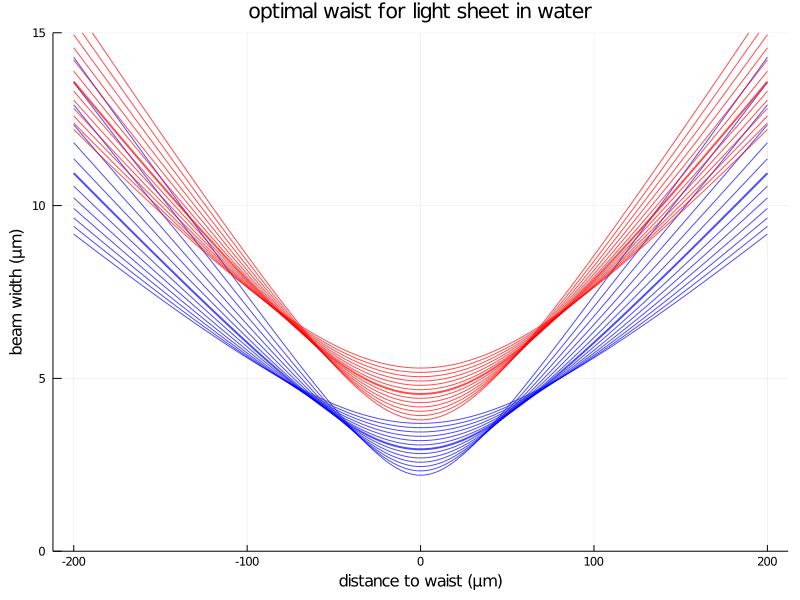
\includegraphics[width=0.8\textwidth]{./files/possible-waist.png}
\caption{On voit ici le profil gaussien à 488 nm et à 915 nm dans l'eau pour différentes valeurs du waist. Le trait épais marque la position optimale pour un faisceau de 400 µm de long.}
\end{figure}

Une valeur de waist possible pour un échantillon de 400 µm est de 3 µm à 488 nm et de 5 µm à 915 nm. Pour ces valeurs, la largeur du faisceau à 488 nm vaut 3 µm au centre et 10 µm sur les bords du cerveau. À 915 nm c'est 5 µm au centre et 14 µm sur les bords mais il faut aussi prendre en compte l'effet deux photons. En pratique, la plupart des neurones sont situés entre -150 µm et +150 µm, la largeur du faisceau aux extrémités n'est donc pas critique.

Pour effectuer le balayage, on déplace le faisceau horizontalement. Pour que l'intensité soit homogène sur une image, il faut adopter une vitesse de déplacement constante. Il est alors possible de faire un aller simple ou des allers-retours en nombre entier pendant le temps d'exposition. Pour obtenir une image volumétrique, il suffit de répéter l'opération pour plusieurs couches, en changeant le plan focal de l'objectif de détection et la position vertical de la nappe. Procéder de cette manière couche après couche force à attendre entre deux couches pour laisser le temps aux éléments mécaniques de se positionner, ce qui prend un temps (~10 ms) non négligeable pour des durées d'exposition courtes. Il est également possible de bouger les éléments mécaniques de manière continue en balayant en aller simple. Les couches sont donc légèrement obliques, mais on gagne considérablement en fréquence d'acquisition. Cela est possible grâce au mode "synchronous readout" de la caméra qui permet de lire les valeurs d'une ligne de pixels tout en exposant une autre.

Pour un temps d'exposition par couche de 10 ms en mode d'acquisition continu, on peut par exemple réaliser un scan du cerveau à 2,5 Hz en 30 couches espacées de 8µm. Cela permet d'imager la majeure partie du cerveau du poisson. Les couches les plus profondes sont moins nettes car le signal traverse plus de tissus avant d'atteindre l'objectif, et la zone située entre les yeux reste dans l'ombre si on n'utilise qu'un laser. Mais chaque neurone visible est imagé à une fréquence de 2.5 Hz.

\section{Microscope miniature rotatif}

Pour étudier le système vestibulaire de la larve de poisson zèbre, une option est de stimuler directement ses otolithes via des pinces optiques [16], une autre est de tourner réellement le poisson pour que la gravité bouge ses otolithes. Cette deuxième solution est plus performante, car elle reproduit réellement la stimulation vestibulaire sans les limitations dues au pinces optiques (manque de calibration, problème d'échauffement...) mais nécessite des développements techniques avancés pour être appliquée sous microscope. En effet, pour conserver le microscope fixe par rapport à un poisson mobile, il faut construire un microscope rotatif, tout en gardant les conditions de stabilité nécessaires à l'imagerie. Depuis 2018, c'est chose faite, Migault \emph{et al} [9] ont développé un microscope à feuille de lumière rotatif capable de mesurer l'activité du cerveau pendant une stimulation vestibulaire réelle.

Pour cela, un microscope à feuille de lumière miniature a été assemblé afin d'être monté sur une plateforme rotative. L'unité d'illumination, composée d'un connecteur de fibre monté sur un positionneur piézoélectrique et de deux objectifs en montage confocal de part et d'autre d'un miroir galvanométrique, tient dans un cube de 10 cm de diamètre. L'unité de détection, composée d'un objectif à immersion monté sur un positionneur piézoélectrique, d'une lentille de tube, d'un filtre coupe-bande, d'un filtre GFP, et d'une caméra, est également très simple, l'élement le plus lourd et encombrant étant la caméra. Le tout pèse environ 2 kg (?) et tient sur une plaque de 50 cm de côté fixée à un moteur à grand couple et grande précision. Lors de la rotation du microscope, l'instabilité de l'imagerie reste inférieure à 500 nm dans la direction verticale et 2 µm dans la direction latérale (cette dernière peut être corrigée lors de l'analyse).

\section{Feuille de lumière deux photons}

Pour étudier le système visuel de la larve, il faut contrôler précisément son environnement visuel. Or un microscope à feuille de lumière classique utilise un laser bleu pour stimuler la fluorescence, et cette longueur d'onde réside dans le domaine visible de la larve de poisson zèbre, ce qui peut l'éblouir et perturber son système visuel. Pour cette raison, Ahrens \emph{et al}, pour l'étude de l'OMR, ont utilisé un microscope à deux photons classique [11]. Cela permet d'illuminer dans l'infrarouge, une longueur d'onde invisible pour le poisson. Cependant ils ne bénéficiaient donc pas des avantages d'un microscope à feuille de lumière et étaient contraints par le balayage point par point à réaliser l'acquisition du cerveau une région après l'autre afin de reconstruire *a prosteriori* l'image du cerveau entier. À peu près en même temps, Truong \emph{et al} publiaient un microscope à feuille de lumière deux photons permettant d'allier les avantages de la microscopie deux photons et de la microscopie à feuille de lumière [17].

Plus tard, Vladimirov \emph{et al} [18] ont montré que l'étude de l'OMR était également possible en microscopie à feuille de lumière un photon, à condition de ne pas éclairer directement l'oeil du poisson. Ils ont utilisé deux feuilles de lumière, l'une éclairant le cerveau par le côté et l'autre par l'avant, entre les deux yeux. Cependant, l'OMR est un réflexe robuste qui ne recourt pas aux fonctions avancées de la vision, et la perturbation due à l'illumination des autres processus visuels n'est pas contrôlée. C'est pourquoi Wolf \emph{et al} ont appliqué la technique mise au point par Truong à l'étude du système visuel de la larve de poisson zèbre [10]. Ils ont construit un microscope à feuille de lumière deux photons et réalisé l'acquisition du cerveau entier lors de stimulations visuelles.

\section{TODO Analyse}

- données volumineuses
- revue de l'existant (CaImAn, suite2P)